\section{탐구 내용}

\subsection{여러 제약조건에서 최적의 확률 분포 탐색}

계를 구성하는 확률분포와 관련하여 여러 제약 조건이 존재할 수 있다. 일단 기본적으로 모든 확률분포가 만족해야하는 조건이 있다. 이는 전사건의 확률이 1이라는 것이다.
\begin{equation}
    \sum_{i} p_{i} = 1
    \label{Constraint1}
\end{equation}

이를 제약조건으로 삼아서 엔트로피를 최대화하는 확률분포를 탐색해보자.
\begin{equation}
    L_{1} = -\sum_{i} p_{i} \ln{p_{i}} - \lambda_{1} ( \sum_{i} p_{i} - 1)
    \label{L_I}
\end{equation}

Lagrange Multiplier Method를 적용하자.

\begin{equation}
    \frac{\partial L_{1}}{\partial p_{i}} = 0:~ -\ln{p_{i}} - 1 - \lambda_{1} = 0, ~p_{i} = \exp{(1+\lambda_{1})}
    \label{Lagrange_I}
\end{equation}

\begin{equation}
    p_{i} = \frac{1}{n}
    \label{p_I}
\end{equation}

즉, 구하는 확률분포는 균일분포(Uniform Distribution)이다. 
% 실제로 $n=2$인 상황을 간단히 생각해보아도 성립함을 볼 수 있다 (그림 \ref{H(X, n=2)}).

% \begin{figure}[H]
%     \centering
%     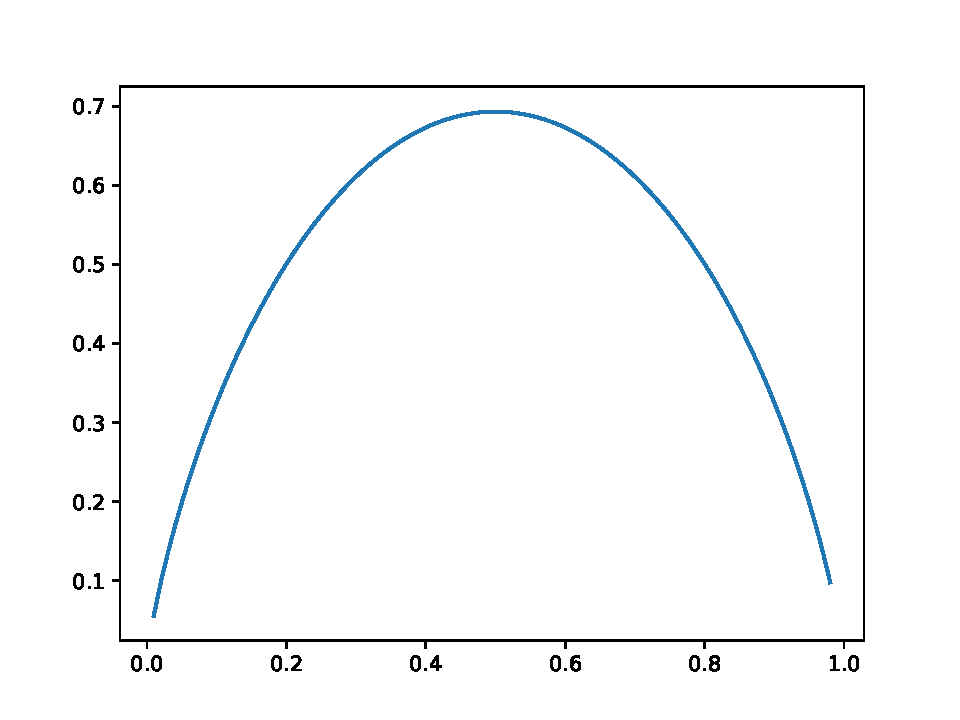
\includegraphics[width=0.45\textwidth]{images/H(X)(coin).pdf}
%     \caption{n=2인 계의 H(X)}
%     \label{H(X, n=2)}
% \end{figure}

그렇다면 계의 확률분포에 대해서 기댓값이 주어진 경우는 어떻게 되는가? 확률분포에 대해서 가장 대중적으로 얻는 값은 기댓값과 표준편차이다. 기댓값이 주어진 경우부터 살펴보자. 사건 $i$에 대응하는 확률변수의 값이 $x_{i}$라고 하자. 또, 주어진 기댓값을 $\mu$라고 한다면 제약조건은 다음과 같다.
\begin{equation}
    \sum_{i} x_{i}p_{i} = \mu
    \label{Constraint2}
\end{equation}

조건 \ref{Constraint1}과 \ref{Constraint2}를 엔트로피에 적용하여 새로운 목적함수를 쓰고 라그랑주 승수법을 적용하면 다음과 같다.

\begin{equation}
    L_{2} = -\sum_{i} p_{i} \ln{p_{i}} - \lambda_{1} ( \sum_{i} p_{i} - 1) - \lambda_{2} (\sum_{i} p_{i}x_{i} - \mu)
    \label{L_II}
\end{equation}

\begin{equation}
    \frac{\partial L_{1}}{\partial p_{i}} = 0:~ -\ln{p_{i}} - 1 - \lambda_{1} - \lambda_{2} x_{i} = 0
    \label{Lagrange_II}
\end{equation}

식 \ref{Lagrange_II}을 정리하면
\begin{equation}
    p_{i} = \exp{(-1-\lambda_{1} - \lambda_{2} x_{i})} = C \exp{(-\lambda_{2} x_{i})}
    \label{p_i(Lagrange_II)}
\end{equation}

의 확률분포를 얻을 수 있다. 이 경우에 $\lambda_{2} \neq 0$이므로 사건 $i$의 확률은 그때의 확률변수 값 $x_{i}$에 대하여 지수함수적으로 비례하고 볼츠만 분포 (Boltzmann Distribution) 이다. 연속 분포에 대해서 제약 조건에 대한 $\lambda_{2}$와 $C$, $\mu$를 구해보면 $C = \lambda_{2} = 1/\mu$임을 알 수 있다 (단, 정의역은 $x>0$으로 제한하였다). 하지만 이산 분포에 대해서는 다르며 $x=1, ~2, ~\cdots, ~n$인 경우를 생각하자.
\begin{equation}
    C(e^{-\lambda}+e^{-2\lambda} + \cdots + e^{-n\lambda}) = 1, ~ \frac{1}{C} = \frac{e^{-\lambda}(1-e^{-n\lambda})}{1-e^{\lambda}}
    \label{C_II}
\end{equation}
\begin{equation}
    C(e^{-\lambda}+2e^{-2\lambda} + \cdots + ne^{-n\lambda}) = \mu
    \label{mu_II}
\end{equation}

식 \ref{C_II}, \ref{mu_II}를 연립하면 다음과 같은 관계식을 얻을 수 있다.
\begin{equation}
    \mu = \frac{1}{1-e^{-\lambda}} - \frac{ne^{-n\lambda}}{1-e^{-n\lambda}}
    \label{mu, n, lambda relation_II}
\end{equation}
이를 풀면 $\mu, n$에 대한 알맞는 $\lambda$를 구할 수 있다. 물리적으로도 기체의 속도 분포를 유도할 때 계의 전체 입자수와 총 에너지가 제한되어 있으며 이는 위의 제약 조건 \ref{Constraint2}와 같다.

% 이산 분포에 대해서는 $\lambda_{2}$를 구할 수 없으며 연속일 때를 가정하겠다. 단, 가능한 Domain은 $x_{i} > 0$이며 이후 시뮬레이션에서는 이를 1, 2, \cdots, 100으로 제한할 것이며 $\lambda_{2} > 0$이어야 하고 연속 가정은 $x$에 대응하는 확률밀도함수를 $p(x)$로 두어 푼다는 의미이다.
% \begin{equation}
%     \int_{0}^{\infty}{C \exp{-\lambda_{2} x} dx} = 1, ~C = \lambda_{2}
% \end{equation}

% \begin{equation}
%     \int_{0}^{\infty}{x C \exp{\lambda_{2} x}dx} = \mu, ~ \mu = 1/\lambda_{2}
% \end{equation}

% 즉, 구하는 분포는 볼츠만 분포와 같은 아이디어를 쓰며 다음과 같다.
% \begin{equation}
%     p(x) = \frac{1}{\mu} \exp{(-\frac{x}{\mu})},~p_i = \frac{1}{\mu} \exp{(-\frac{x_{i}}{\mu})}
%     \label{p_II}
% \end{equation}


통계학적으로 분석을 할 때는 기댓값 뿐만이 아니라 표준편차도 중요하다. 표준편차가 $\sigma$로 주어진 경우를 살펴보자.
\begin{equation}
    \sum_{i} p_{i}x_{i}^{2} - \mu^{2} = \sigma^{2}
    \label{Constraint3}
\end{equation}
이 경우의 목적함수는 다음과 같다.

\begin{equation}
    L_{3} = -\sum_{i} p_{i} \ln{p_{i}} - \lambda_{1} ( \sum_{i} p_{i} - 1) - \lambda_{2} (\sum_{i} p_{i}x_{i} - \mu) - \lambda_{3}(\sum_{i} p_{i}x_{i}^{2} - \mu^{2} - \sigma^{2})
    \label{L_III}
\end{equation}
라그랑주 승수법을 적용하면
\begin{equation}
    \frac{{\partial L_{3}}}{\partial p_{i}} = 0:~ -\ln{p_{i}} - 1 - \lambda_{1} - \lambda_{2} x_{i} - \lambda_{3} x_{i}^{2} = 0
    \label{Lagrange_III}
\end{equation}
\begin{equation}
    p_{i} = \exp{(-1-\lambda_{1} - \lambda_{2} x_{i} - \lambda_{3} x_{i}^{2})} = A \exp{(-\lambda_{3} (x_{i} - B)^{2})}
    \label{p_i(Lagrange_III)}
\end{equation}

이는 가우스 분포 (Gaussian Distribution)이다. 역으로 $D_{KL}(P||Q)$를 이용하여 가우스 분포는 주어진 제약 조건 (식 \ref{Constraint3})에서 $H(p)$가 제일 큰 확률분포임을 알 수 있다. 일반적으로 주어진 모수 $\mu,~\sigma$에 대한 확률분포함수는 다음과 같음을 알고 있다.
\begin{equation}
    p(x) = \frac{1}{\sigma\sqrt{2\pi}}\exp{(-\frac{1}{2}(\frac{x-\mu}{\sigma})^{2})}
\end{equation}
하지만 역시나 이산적인 경우에 대해서 계산을 해주어야 하고 $x=1, ~2, ~\cdots, ~n$인 경우를 생각한다.
\begin{equation}
    A e^{-\lambda (1 - B)^{2}} + A e^{-\lambda (2 - B)^{2}} + \cdots + A e^{-\lambda (n - B)^{2}} = 1
\end{equation}
\begin{equation}
    A e^{-\lambda (1 - B)^{2}} + 2A e^{-\lambda (2 - B)^{2}} + \cdots + nA e^{-\lambda (n - B)^{2}} = \mu
\end{equation}
\begin{equation}
    A e^{-\lambda (1 - B)^{2}} + 2^2 A e^{-\lambda (2 - B)^{2}} + \cdots + n^2 A e^{-\lambda (n - B)^{2}} = \mu^2 + \sigma^2
\end{equation}

위 세 식으로부터 $A$, $B$, $\lambda$를 $\mu, ~\sigma$로 나타내는 것이 목표였으나 사실상 불가능하다. 그나마 얻을 수 있는 관계식은 $\lambda$로 편미분하여 정리할 시 얻어지는
\begin{equation}
    \ln{A} = \lambda((B-\mu)^{2}+\sigma^{2}) + (const)
\end{equation}

이지만 이로는 부족하며 정확한 상수는 알 수 없다.

\subsection{시뮬레이션}

결국 문제의 본질은 주어진 제약 조건 하에서 엔트로피 값을 최대화할 수 있는 확률 분포를 찾는 것이며 이는 최적화 문제로 분류할 수 있다. 이러한 최적화 문제를 해결하는데 대표적인 방법으로는 유전적 알고리즘(이하 GA)가 존재한다. 따라서 본 프로젝트에서는 이 방식을 활용하여 수식 유도의 결과와 실제 최적화 결과가 일치하는지 검증해보고자 한다.

먼저, GA에 대해 알아보자. GA는 다윈의 자연선택설에 기반하여 더 적합도가 높은 유전자들이 확률적으로 더 많이 살아남도록 하고 살아남은 우수한 유전자들끼리 서로 조합하여 더 나은 유전자를 가진 다음 세대를 만든다. 그리고 이 과정을 반복함으로써 최종적으로 최적해를 찾는다. GA를 구성하는 단계로는 초기 유전자 생성, 평가, 교차, 돌연변이가 있으며 본 프로젝트에서 차용한 GA의 연산들은 아래와 같다.

\newpage
\textbf{1. 초기 유전자 생성}

먼저, GA를 통해 확률분포를 최적화하는 것이 목표이기 때문에 이를 유전자로 표현해야 한다. 때문에 확률변수 $X$: $x_i = 1, 2, 3, \cdots, 20 ~(n=20)$에 대하여 각각의 확률 $p_i$를 유전자로 잡았다. 즉, 유전자는 $n=20$인 확률 분포가 되는 것이다.
\begin{equation}
    gene = \{ p_i : 1 \leq i \leq 20\}
    \label{gene}
\end{equation}

한 세대는 750개의 유전자로 구성되어 있으며, 초기 유전자의 경우 합이 1이 되는 랜덤한 실수쌍 10개로 생성하였다.\\

\textbf{2. 평가}

우리가 찾고자 하는 확률 분포는 다음 네 가지 조건을 만족해야 한다.
\begin{itemize}
    \item $\sum_i{p_i} = 1$ (조건 I)
    \item $H(X) = -\sum_i{p_i \ln{p_i}}$를 최대화
    \item $\mathbb{E}[X] = \mu_0$ (조건 II)
    \item $\sigma(X) = \sigma_0$ (조건 III)
\end{itemize}

따라서 평가함수는 이러한 제약 조건들을 반영해야 한다. 다만, 첫 번째 제약 조건의 경우 유전자의 생성 단계에서 고려하여 평가함수에는 반영하지 않도록 하였다. 그 결과 최종적으로 짠 평가함수는 식 (\ref{eq:fitness})과 같다.

\begin{equation}
    \label{eq:fitness}
    fitness = w_1 \times e^{H(X)^2} + w_2 \times \frac{1}{1+(\mathbb{E}[X]-\mu_0)^2} + w_3 \times \frac{1}{1+|\sigma(X)-\sigma_0|}
\end{equation}

각 항에 대해 살펴보면, 첫 번째 항은 $H(X)$를 최대화하기 위함이고, 두 번째 항은 $\mathbb{E}[X]=\mu_0$가 되도록 하기 위해 그 차이가 줄어들수록 값이 커지게 하였고, 세 번째 항은 $\sigma(X)=\sigma_0$는 두 번째 항과 마찬가지 원리로 참값과 가깝게 되도록 한 것이다. 다만, 표준편차의 경우 애초에 그 값과 멀리 떨어진 값에서 출발한 경우가 많아 0으로 수렴할 여지가 다분하여 좀 더 차이가 클 때 적게 반영되도록 절댓값으로 잡게 되었다. 또한, 제약조건이 필요없는 경우 해당 제약조건의 가중치($w_i$)를 0으로 잡아 이가 반영되지 않도록 하였다.\\

\textbf{3. 교차 \& 돌연변이}

새로운 유전자를 생성하는 단계로, 기존의 있던 유전자들을 적합도에 비례하는 확률로 선택하여 해당 유전자끼리 조합하여 다음 유전자를 만들게 된다. 이때, 실제 유전자의 교차 과정을 모방하여 한 지점을 기준으로 그 앞은 부모 1의 유전자, 그 뒤는 부모 2의 유전자를 따르도록 하였다. 또한, 수렴 직전의 상황에서도 더 좋은 유전자가 잘 선택되게 하기 위하여 선택압을 4배로 맞추어, 가장 안 좋은 해와 좋은 해가 선택될 확률이 4배가 되도록 하였다.
교차 이후 유전적 다양성을 확보하기 위하여 일정 확률로 4개 이하의 $i$를 선택하여 각 $p_i$가 $\pm 50\%$의 범위 내에서 변하도록 하였다. 그리고 최종적으로 조건 Ⅰ을 만족시키기 위하여 전체 확률 합이 1이 되도록 비례배분하게 된다.

이 과정을 수식적으로 표현하면 아래와 같다. 부모 유전자 $gene_1$과 $gene_2$를 룰렛 알고리즘을 통해 선택하여 자식 유전자 $gene'$을 만든다고 할 때, $k$번째를 기준으로 교차 연산을 거치면 

\begin{equation*}
    p'_{i, 0} = \begin{cases}
        p_{1, i} & \text{if $\; 0 \leq i \leq k$}\\
        p_{2, i} & \text{if $\; k < i < 20$}
    \end{cases}
\end{equation*}

과 같이 된다. 그리고 변이를 받을 대상의 인덱스를 모은 집합을 $S$라 둘 때, 각 $p'_{i, 0} (i \in S)$에게 $w_i (-0.5 \leq w_i \leq 0.5)$만큼의 변이를 주게 된다면 유전자는 다시 아래와 같이 바뀌게 된다.

\begin{equation*}
    p'_i = \begin{cases}
        (1+w_i) p'_{i, 0} & \text{if $i \in S$}\\
        p'_{i, 0} & \text{else}
    \end{cases}
\end{equation*}

그리고 이렇게 생기게 된 유전자들을 최종적으로 합이 1이 되도록 하기 위하여 합으로 나눠주게 되면 새로운 자식 세대 유전자가 된다.